% !TEX root = /home/weznon/programming/0207Programming/ftc-programming-guide/main.tex

\documentclass[../main.tex]{subfiles}

\begin{document}
\newpage
%Begin the stuff!
%This version of the template has some placeholder stuff so you can see what it looks like
\section{Vision}
While this really should go under sensors, it is a big enough category to warrant a section for itself.

\subsection{What is it}
We have previously discussed various sensors. However, the limitation inherent with all of them is the fact that they are all highly specialized with specific target ranges. The primary advantage of vision systems is that they offer a much larger range of view.
\subsection{OK but why do I need it}
\subsection{Vuforia}
\subsection{PixyCam}
\begin{figure}[H]
    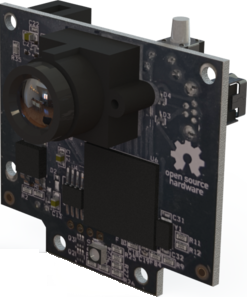
\includegraphics{sections/vision/images/pixy.png}
    \caption{A PixyCam, so you know what it looks like.}
\end{figure}
PixyCam is another vision system. It provides object recognizing capability by grouping together various pixels of a similar color. The color, thresholds, etc. can be set using a program you install on your computer. The main takeaway from this is that the Pixy is best suited to identifying objects of a roughly uniform color, based on the presence of that color in the image it sees.

TOOD: Insert some pictures of the training thing here. Requires using a pixy

We do not have example code for using a PixyCam, since we have never used it on our robot. This is for a couple of reasons. The first of which is that PixyCam is INCREDIBLY susceptible to lighting changes. It is highly likely that on competition day your settings will not work, depending on the lighting conditions at the meet. The second is that even when under proper settings, it isn't that great. It uses RGB, which is not the greatest for color detection. It has tons of false positives and noise, and all around isn't great. It works best on bright colors - the particles/jewels from Velocity Vortex/Relic Recovery, the relic from Relic Recovery, and the gold mineral from Rover Ruckus would work well. The glyphs from Relic Recovery worked horribly. 

\subsubsection{TL;DR}
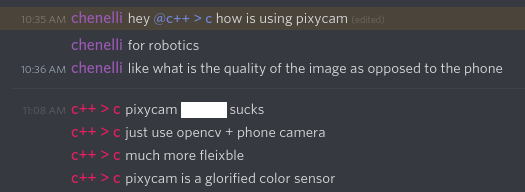
\includegraphics[width=400pt]{sections/vision/images/2019-02-27-195334_3840x1080_scrot_cropped.png}

\subsection{Tensorflow}
Tensorflow is an interesting vision system. The premise is this; there is some neural network trained to identify different pieces present in the game. This was first done in the Rover Ruckus season, as since I am currently writing this while that season takes place, I don't know whether it will be done again, as FTC trained the model to detect the minerals themselves. It is something you could do yourself, TODO: GET TANAY TO TALK ABOUT THIS PART
\begin{figure}[H]
    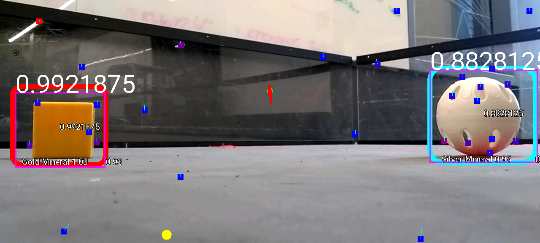
\includegraphics[width=400pt]{sections/vision/images/tensorflowOutput.png}
    \caption{Sample output of the Tensorflow. Each object that it believes to be a trained object, in this case the minerals, is boxed. Next to each box is a number, representing how confident the neural network is that the box is a mineral. In the FTC SDK, methods for getting the location of the box, confidence, and type of identified object the box contains are exposed}
\end{figure}

So, what does this look like from a programming standpoint? A full teleop which implements the Tensorflow identification (at least for the 2018-2019 season) can be found in TODO: figure out appendixes.

For now, assume that \verb|tfod| is a standard Tensorflow object provided by the FTC SDK.

\begin{lstlisting}[language=Java]
\end{lstlisting}
\subsection{OpenCV}
\end{document}
